\section{Results and discussion}
% Define a custom command to create sections with shared structure

As explained in \ref{sec:methodo}, the first objective is to effectively post-process a single NWP forecast model, by benchmarking the models altogether. 

The following step will be to look at the results in the details to prove the true effectiveness of the post-processing.
\subsection{Post-processing of a single forecasting NWP model}
\subsubsection{Study of the models altogether} 
\paragraph{MAE}
\begin{figure}[htb!]
    \centering
    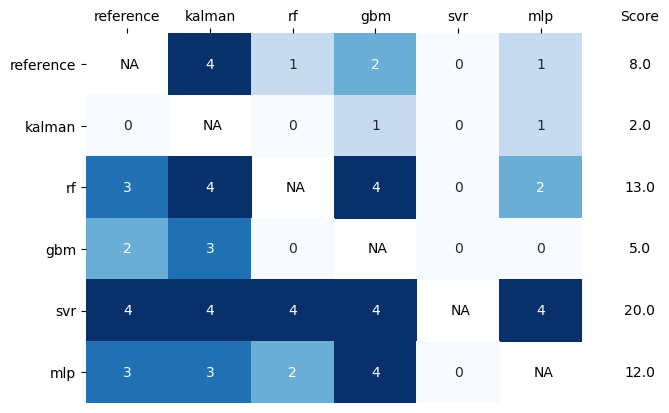
\includegraphics[width=\columnwidth]{figures/first_study/significance_matrix_mae.png}
\caption{Significance matrix for MAE. The value $V_{(i,j)}$ of the $(i,j)$ cell indicates how often the model of line i performs better than the one of column j, across the 
4 sites. For example, the MAE of the MLP model post-processed data is 3 times lower than the MAE of the reference model, and for 1 site (4 - 3 = 1), it is higher.}
\end{figure}

\begin{figure}[htb!]
    \centering
    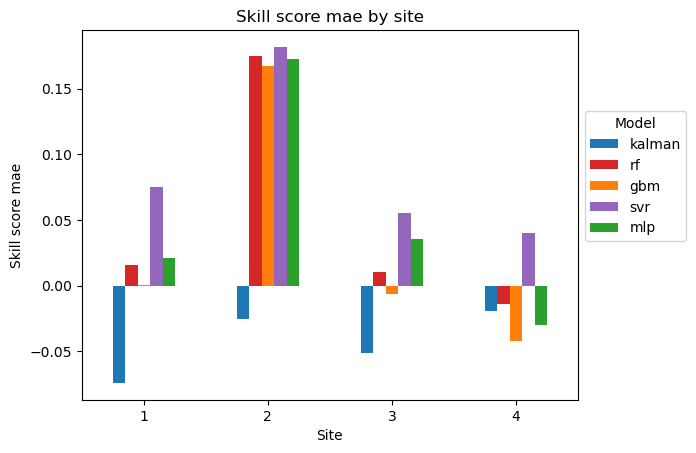
\includegraphics[width=\columnwidth]{figures/first_study/ss_mae.png}
    \caption{MAE skill score plot across the 4 sites.}
\end{figure}
\paragraph{RMSE}

\begin{figure}[htb!]
    \centering
    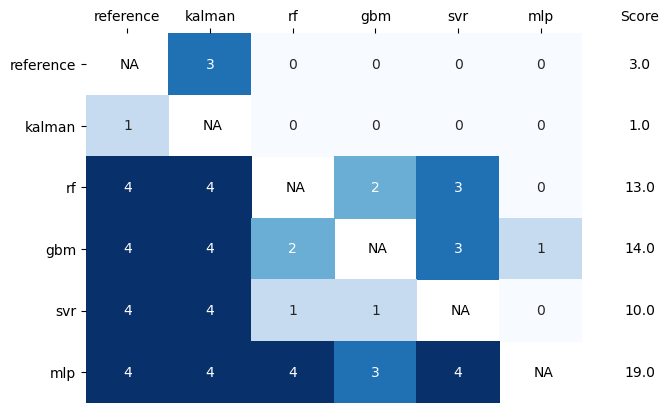
\includegraphics[width=\columnwidth]{figures/first_study/significance_matrix_rmse.png}
\caption{Significance matrix for RMSE. The value $V_{(i,j)}$ of the $(i,j)$ cell indicates how often the model of line i performs better than the one of column j, across the 
4 sites. For example, the RMSE of the MLP model post-processed data is 3 times lower than the RMSE of the reference model, and for 1 site (4 - 3 = 1), it is higher.}
\end{figure}

\begin{figure}[htb!]
    \centering
    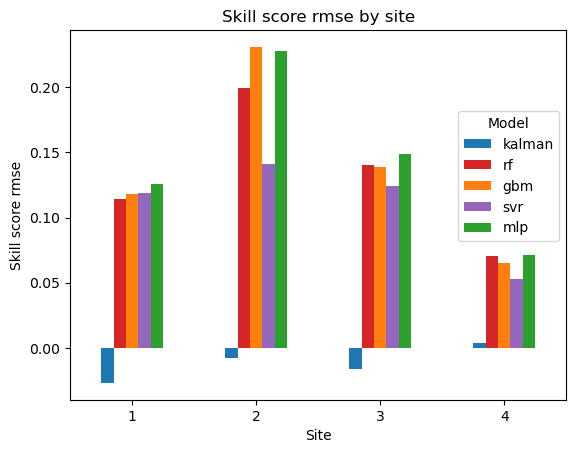
\includegraphics[width=0.75\columnwidth]{figures/first_study/ss_rmse.png}
    \caption{RMSE skill score plot across the 4 sites.}
\end{figure}

\subsubsection{Detailled study of the most performing model}
With the aim of clarity, only the plots of the single site 2 will be shown here.
The overall similarity of the results across the 4 sites also motivate this choice.

The ones of the other sites can be found in the appendix to fortify the belief in the analysis drawn for a single site.

\paragraph{MAE}
\begin{figure}[htb!]
    \centering
    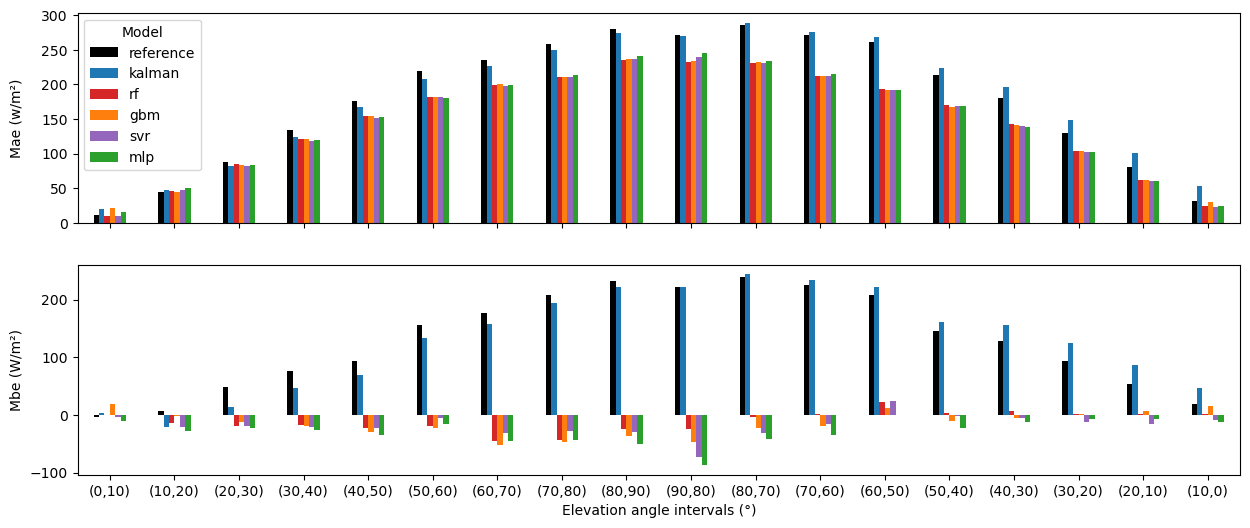
\includegraphics[width=\columnwidth]{figures/first_study/mae_mbe_site2.png}
\caption{MAE and MBE levels across all elevation angle intervals of a day, for site 2.}
\end{figure}

\begin{figure}[htb!]
    \centering
    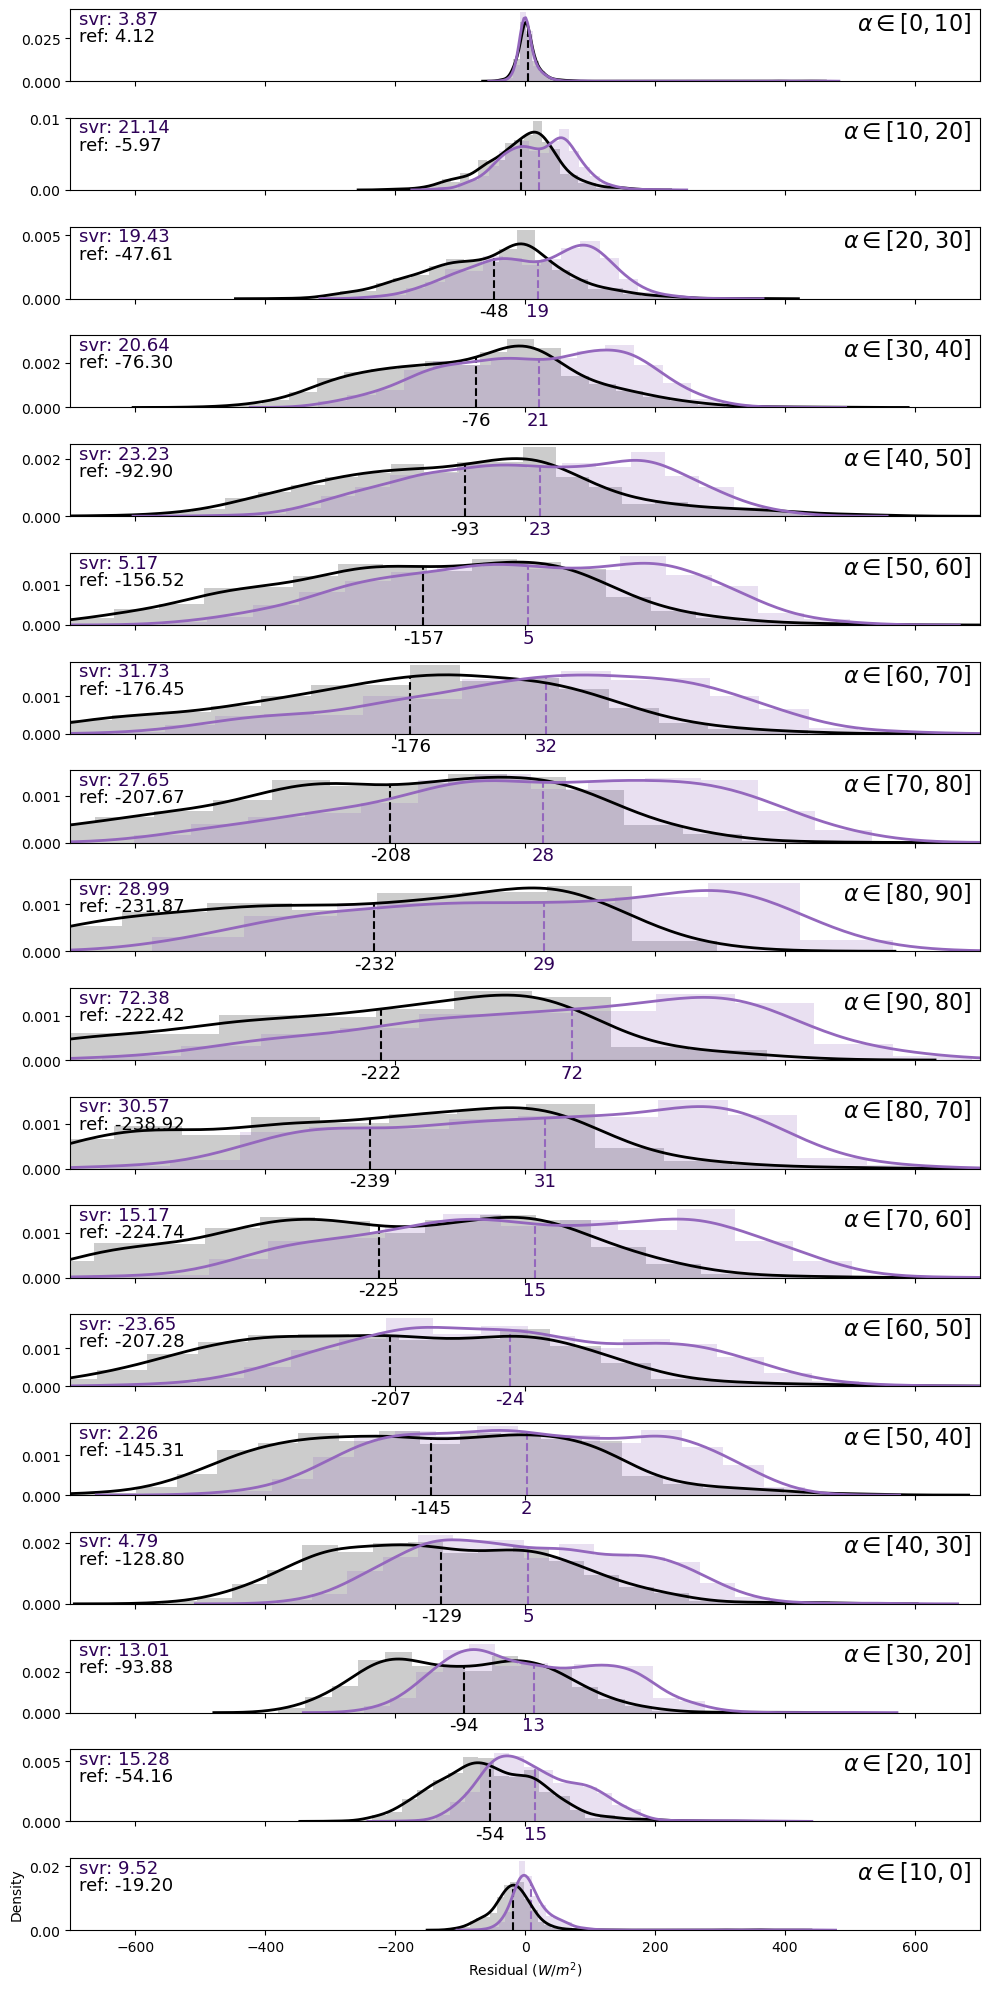
\includegraphics[width=\columnwidth]{figures/first_study/residual_errors_svr_site2_mae.png}
\caption{Residual error levels across all elevation angle intervals of a day, for a SVR model, for site 2.}
\end{figure}


\paragraph{RMSE}
\begin{figure}[htb!]
    \centering
    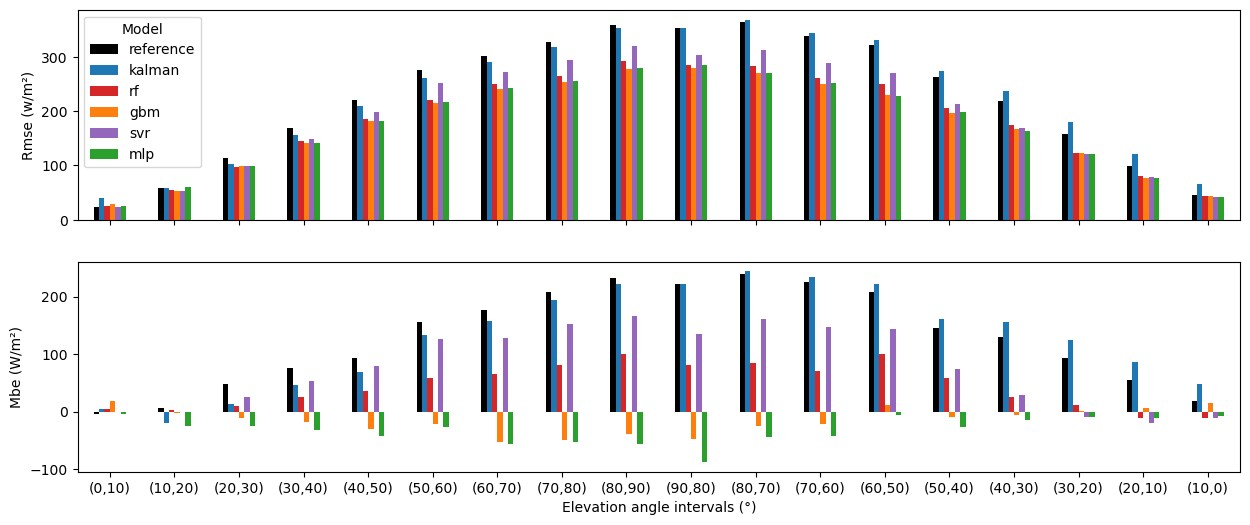
\includegraphics[width=\columnwidth]{figures/first_study/rmse_mbe_site2.png}
\caption{RMSE and MBE levels across all elevation angle intervals of a day, for site 2.}
\end{figure}

\begin{figure}[htb!]
    \centering
    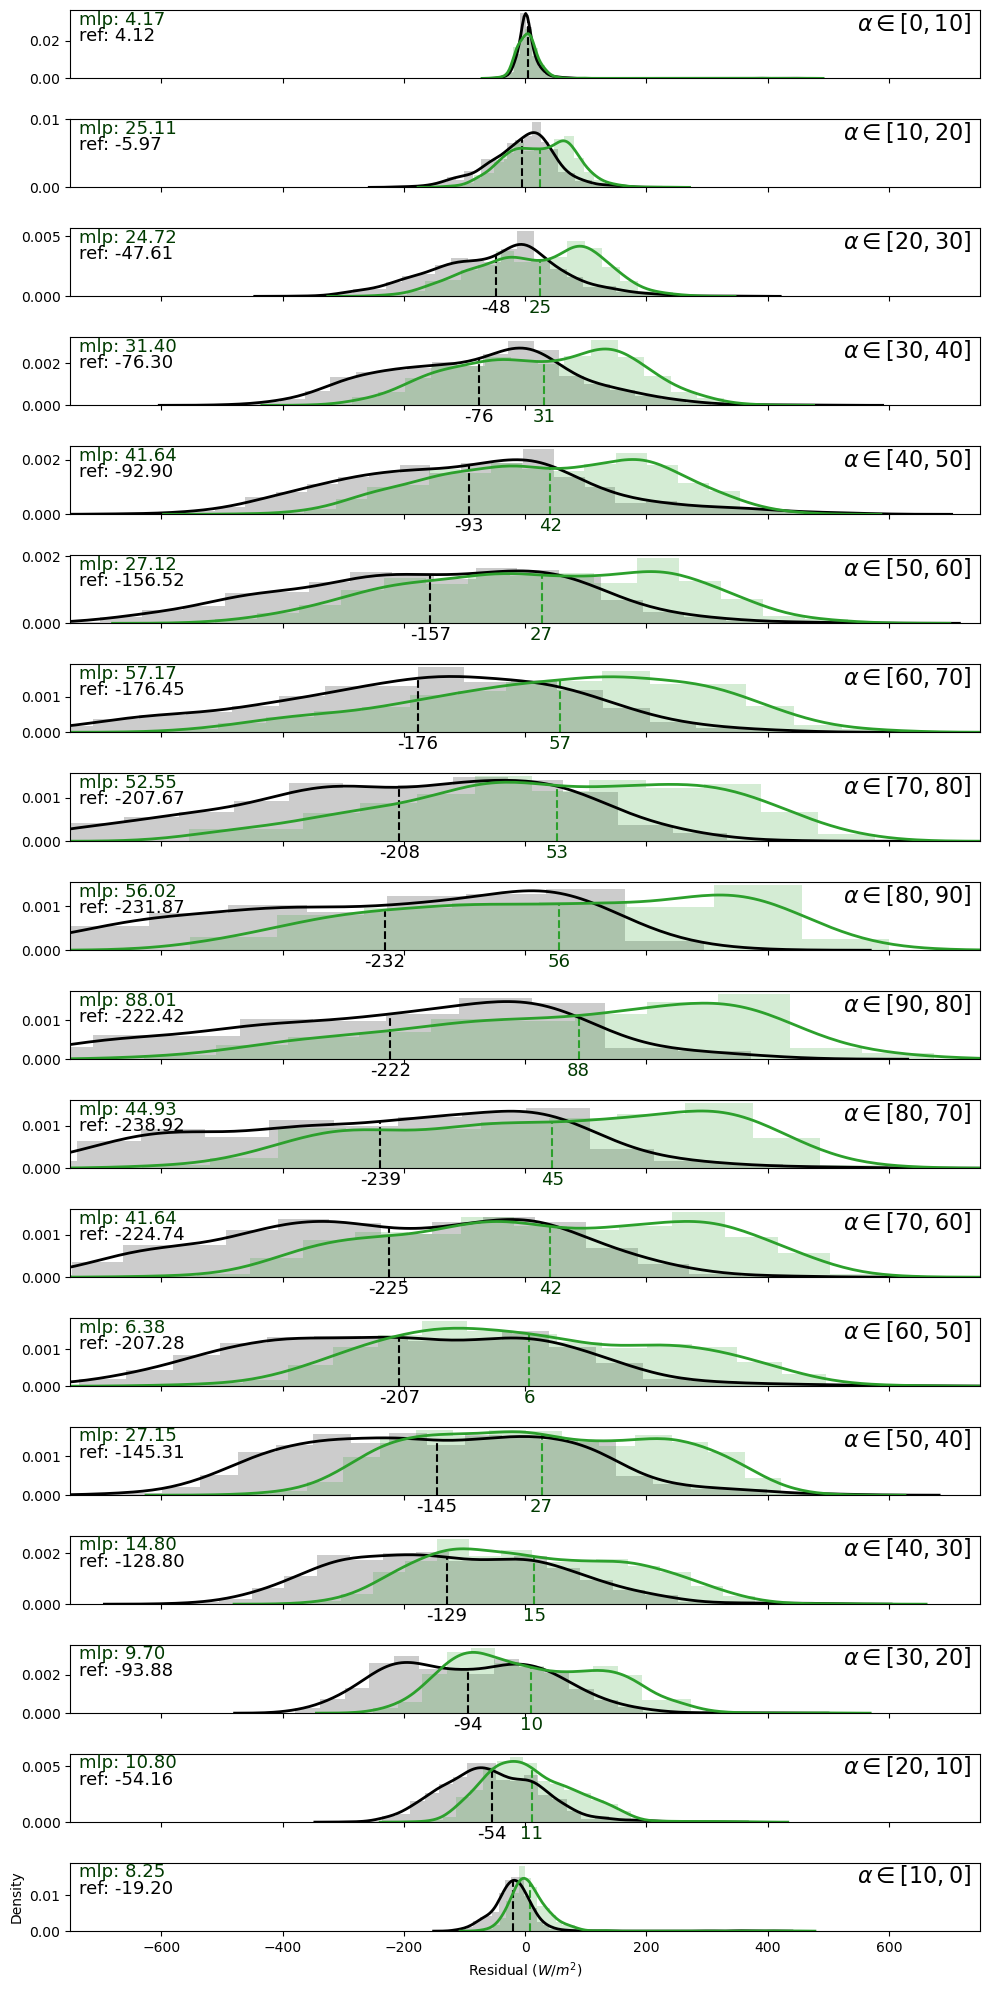
\includegraphics[width=\columnwidth]{figures/first_study/residual_errors_mlp_site2_rmse.png}
\caption{Residual error levels across all elevation angle intervals of a day, for a MLP model, for site 2.}
\end{figure}

\subsubsection{Sensitivity study}
It is also necessary to perform a sensitivity study of the parameters that are not tuned in our process. It is why the influence of the choices of predictors, of learning periods 
and of forecasting model are successively performed. 

With the aim of clarity, the results will be here presented with the MAE optimisation, but the results of the RMSE optimisation lead the same conclusions, and can also
be found in the appendix.

\paragraph{Influence of the choice of the predictors}
\begin{table}[htb!]
\begin{center}
\begin{tabular}{|l|llll|}
\toprule
{} &  0 &  1 &  2 &  3 \\
\midrule
$ghi_{GFS}$            &  X &  X &  X &  X \\
$temperature^{2m}_{GFS}$ &  X &  X &    &    \\
$\theta$             &  X &  X &  X &    \\
$\phi$            &  X &  X &  X &    \\
$ghi_{cs}$             &  X &    &  X &    \\
\bottomrule
\end{tabular}
\end{center}
\label{tab:pred_configs}
\caption{Description of the configurations of the sets of predictors.}
\end{table}

\begin{figure}[htb!]
    \centering
    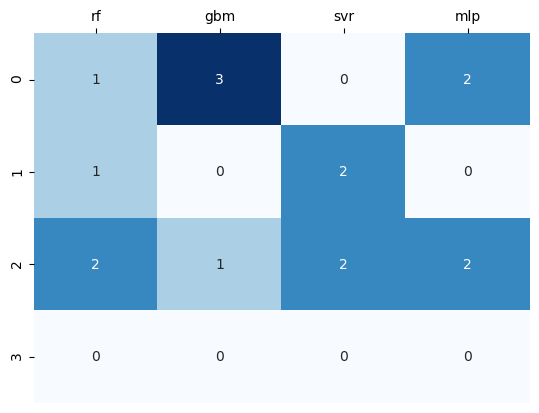
\includegraphics[width=\columnwidth]{figures/first_study/comp_predictors_mae.png}
\caption{Pairwise systematicity matrix for MAE. The value $V_{i,j}$ of
 the cell $(i,j)$ indicates how often the configuration of line i is the best one, across 
 the 4 sites, for the model of column j. For example, the configuration 0 is the best one
 with a GBM post-processing for 3 sites, and the configuration 2 is the best one for 1 site.}
\end{figure}

\begin{figure}[htb!]
    \centering
    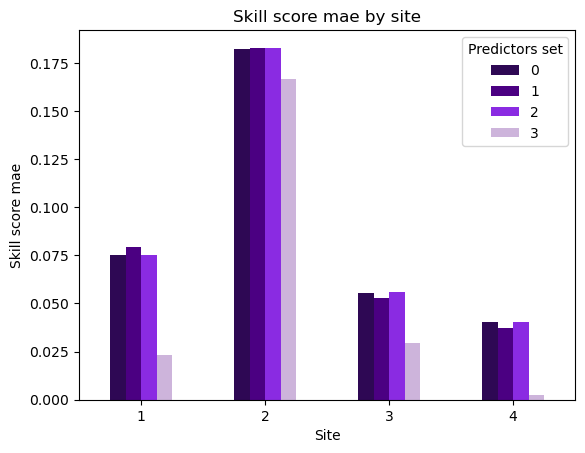
\includegraphics[width=\columnwidth]{figures/first_study/comp_predictors_mae_svr.png}
\caption{Comparison of the MAE skill scores of the different configurations.}
\end{figure}

\paragraph{Influence of the learning period}

\subsection{Benchmarking the linear regression models}
\subsection{Showcase of the hybrid model}